\chapter{Computational methods}
\label{ch:Computational methods}
In this section, a number of computational methods that can be used for conceptual structural design are introduced. 

\section{Form-Finding}
Physical models or numerical simulations can be used for form-finding, which aims to find the form of a structure under load where some static equilibrium is satisfied. The static equilibrium corresponds to a structure that can support the applied load using only compression or tension, and is thus a very efficient structure. For physical models, a hanging chain or cloth can be used to find the static equilibrium.

The different form-finding methods can be divided into three major categories \cite{Veenendaal2012a}: 

\begin{itemize} 
\item Stiffness matrix methods based on elastic and geometric stiffness matrices. These methods have been adapted to structural analysis for form-finding.
\item Geometric stiffness methods. These material-independent methods include the force density method \cite{Schek1974}, which uses the ratio of force to length. Several other methods have been developed by extending this approach.
\item Dynamic equilibrium methods. These methods find the steady-state equilibrium through use of dynamical modeling. One such method is dynamic relaxation \cite{Day1965}, which is explained in further detail in Section \ref{sec:dr}.
\end{itemize} 

\begin{figure}
  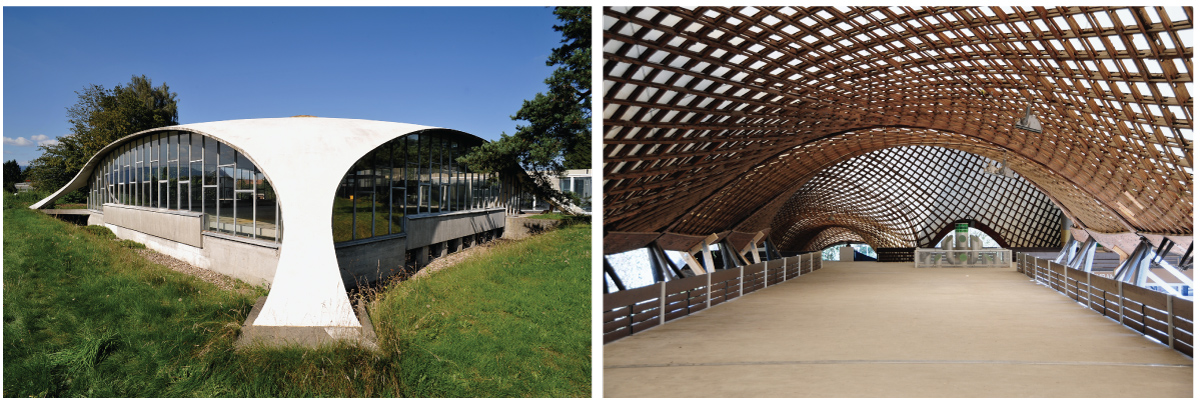
\includegraphics[width=380pt]{graphics/formfinding-ex.jpg}
  \caption{Example of form-found structures. Left: Concrete dome by Heinz Isler, © Chriusha, Wikimedia Commons; Right: Multihalle in Mannheim by Frei Otto © Hubert Berberich, Wikimedia Commons}
  \label{fig:Stevin}
\end{figure}

\subsection{Dynamic relaxation}
\label{sec:dr}
Dynamic relaxation involves solving a set of nonlinear equations. The method computes the movement of a structure over time to find the static equilibrium between the internal and external forces \cite{Day1965, barnes1988form}. 

In each time step  $\Delta t$, the internal forces ,$f_{int}$, for all elements are computed from the nodal displacements $u$. A residual $R$ can be computed as

\begin{equation*}
  R = f_{ext} - f_{int} 
\end{equation*}

where $f_{ext}$ represents the external forces acting on the structure. Using Newton’s second law, the acceleration (time derivative of the velocity) can be computed for node $i$ in the $x$-direction at time $t$ as

\begin{equation*}
  R^t_{ix} = M_i  \cdot \dot{v}^t_{ix}
\end{equation*}

where $M_i$  is a lumped, fictitious mass at node $i$. To enforce suitable boundary conditions, the residual is set to zero for the corresponding degrees of freedom. With the time step known, the velocity of node $i$ in the $x$-direction can be computed using a finite difference method:

\begin{equation*}
  v^{t+\Delta t}_{ix} = v^{t-\Delta t}_{ix} + \frac{\Delta t}{M_i} \cdot R^t_{ix}
\end{equation*}

With this velocity, the updated geometry can be determined as

\begin{equation*}
  x^{t+\Delta t}_{ix} = x^t_i + \Delta t \cdot v_{ix}^{t-\Delta t / 2}
\end{equation*}

Once the geometry has been updated, this iteration is complete and the computations start over by computing the new residual. The geometry is modified in each iteration until an equilibrium is reached between the external and internal forces. Viscous or kinetic damping is often used to aid convergence \cite{barnes1988form}.

A formulation that combines CAD-geometry and dynamic relaxation \cite{Alic2015} for form-finding has recently been developed.

\section{Optimization methods}
Michell pioneered the field of structural optimization, and in 1904 published a series of results using minimum-weight Michell trusses \cite{Michell1904}. These trusses are still used today as benchmarks for topological optimization with framed trusses \cite{Clune2013}. 

Structural optimization is a numerical method that finds the best solution for a mathematically formulated objective function subject to a set of constraints. The following variables are always present in structural optimization \cite{christensen2008introduction}:

\begin{itemize} 
\item \textit{Objective function (f) }- A function that classifies designs with respect to a quantifiable objective. This function returns a numerical value that represents the quality of the design regarding one or more criteria. Usually, a smaller function value is better, i.e., a minimization problem. Frequently, $f$ measures the weight, maximum displacement, strain energy, or cost of a design.
\item \textit{Design variable (x)} – A vector that describes the design with numerical values, the design variable often represents the topology, nodal positions, cross-sectional area, or material.
\item \textit{State variable (y)} – For a given design with the design vector $x$, the state variable $y$ represents the response of the structure, i.e., how well the structure performs in terms of the evaluated criterion.
\end{itemize} 

The optimization problem can now be described as follows \cite{christensen2008introduction}:

\begin{equation}
SO=\begin{cases}
    \textrm{minimize } f(x,y) \textrm{ with respect to } x \textrm{ and } y \\
    {\textrm{subject to} \begin{cases}
        \textrm{behavioral constraints on } y\\
        \textrm{design constraints on } x\\
	\textrm{equilibrium constraints} \\
    \end{cases}}
      \end{cases}
    \end{equation} 


Various optimization methods have been developed, and the best method for any one problem will depend on the associated solution space. A problem can also have multiple objective functions, i.e., multi-objective optimization, which can be formulated as follows:

\begin{equation*}
minimize(f_1(x,y),f_2(x,y), \dotsc, f_n(x,y))
\end{equation*}

This is not a standard optimization problem, as the objective functions are optimized for the same design variables. Instead, a so-called Pareto optimality is sought, where there is no other design that better satisfies all the objectives \cite{christensen2008introduction}. If no single Pareto optimal point exists, a Pareto front can be found in some objective space that has different objectives on the axes, e.g., structural efficiency, operational energy consumption, sunlight.

\subsection{Gradient-based methods}
\begin{figure}
  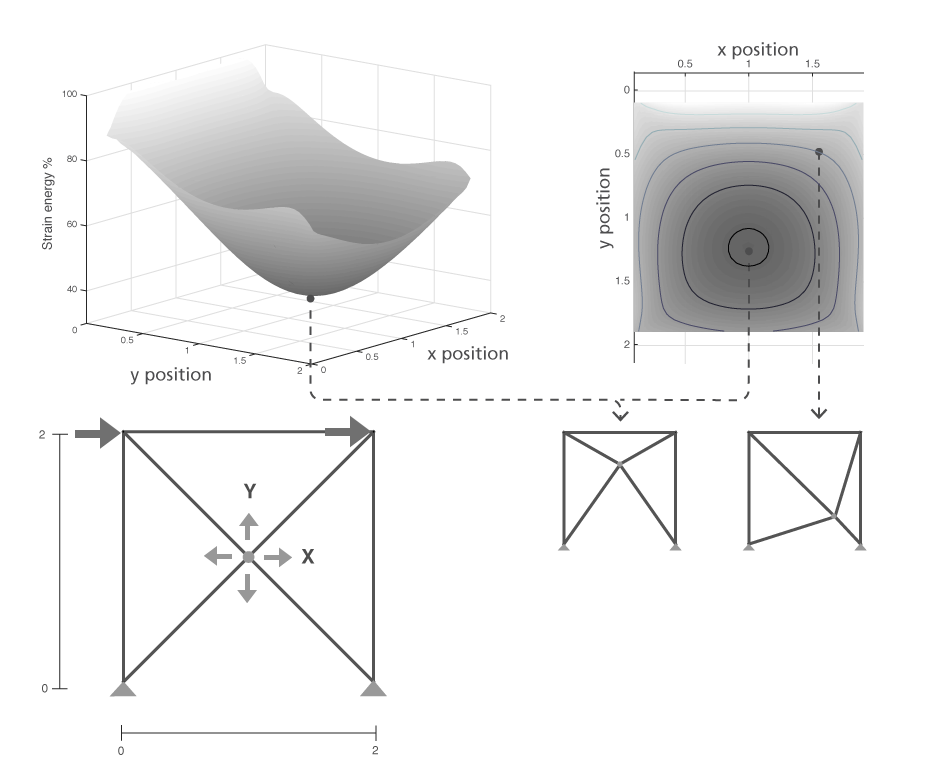
\includegraphics[width=310pt]{graphics/designspace.png}
  \caption{Design space for a shape optimization problem}
  \label{fig:designspace}
\end{figure}

Gradient-based methods make use of the first and/or second derivative of the objective function to iteratively converge towards a solution. These methods are fast, consistent, and their results are repeatable (no randomness). However, the solution space of the objective function must be convex (such as the design space in Figure \ref{fig:designspace}), continuous, and at least once-differentiable. The problem with using such methods for engineering and design is that many of the scenarios are messy \cite{schlaich2006challenges} in that they have non-convex solution spaces that contain multiple local optima. Examples of gradient-based techniques include steepest descent and the Newton--Raphson method \cite{christensen2008introduction}. 

\subsection{Evolutionary algorithms}
Evolutionary algorithms are a collection of generic population-based heuristic optimization algorithms \cite{Bangert2012}. These algorithms are inspired by biological evolution, survival of the fittest, and natural selection. The solvers introduce a degree of randomness to search the solution space, which improves the ability to find global optima.

One of the best-known and most widely used algorithms in this category is the genetic algorithm \cite{Goldberg1989}, which is inspired by biological evolution. This algorithm has the benefits of being robust, guaranteeing a solution, and not requiring a differentiable objective function. 

\begin{figure}
  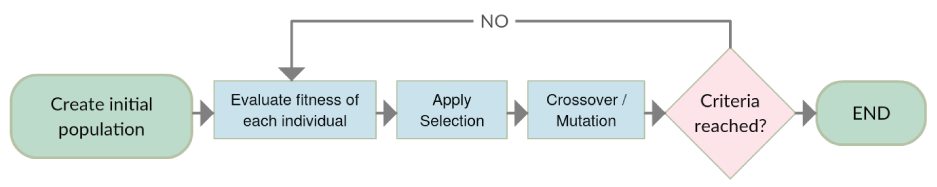
\includegraphics[width=310pt]{graphics/ga.png}
  \caption{Genetic Algorithm procedure}
  \label{fig:ga}
\end{figure}


The genetic algorithm can be described as follows (see Figure \ref{fig:ga}):

\begin{enumerate} 
\item \textit{Create initial population }– First, an initial population is created, either at random or through some type of sampling (e.g., Latin hypercube sampling \cite{10.2307/1268522}).
\item \textit{Evaluate fitness of each individual} – The objective function is evaluated to assign a score (heuristic) to each individual.
\item \textit{Apply selection} – Individuals with higher fitness scores have a better chance of being selected for crossover, a metaphor for mating.
\item \textit{Crossover/Mutation} – The individuals with higher fitness scores recombine their properties (in this context, design variables) with each other to create a new generation. Introducing a small chance of mutation, or random change, when two individuals crossover reduces the risk of the algorithm becoming trapped around a local optima. Elitism can be introduced to allow the best performing individuals to move to the next generation, which can improve convergence. 
\item \textit{End} – The procedure continues until a preselected criterion is reached, often the maximum number of generations or when the solution has converged.
\end{enumerate} 


One weakness of the genetic algorithm is that it can be computationally expensive, as the objective function must be called for each new individual. There is also a lot of fine tuning involved with the different types and rates of crossovers, mutations, and other parameters. 

Genetic algorithms have the benefit that multiple strong solutions can be presented to the user (different individuals from the population). This can be used in conceptual design, where an aesthetically attractive, well-performing solution is sought. The algorithm can also be used for interactive optimization \cite{Scott2002}, whereby a user can intervene in the selection process to move the population in the desired direction. Genetic algorithms have also been extended to multi-objective optimization, where the population converges to the Pareto front \cite{deb2002fast}.

\subsection{Topological optimization}
To optimize the material layout for a given a set of boundary conditions and external forces, topological optimization can be used. This method can be implemented through the use of finite element analysis combined with optimization methods \cite{bendsoe2009topology}. However, the resulting optimal material layout can be highly complex, making it infeasible to actually build.

\section{Eigenvalue analysis}
Eigenvalue analysis can be used to find the dynamic or static modal shapes of a structural model. From the stiffness matrix $\mathbf{K}$ of a structure, a set of scalar stiffness values can be determined \cite{Olsson2003}. Assume that the set of displacements $\mathbf{a}$ is proportional to a corresponding set of forces $\mathbf{f}$, i.e.,

\begin{equation*}
\mathbf{f} = \lambda \mathbf{a}
\end{equation*}

This can be combined with a linear elastic finite element formulation, i.e.,

\begin{equation*}
\mathbf{Ka} =\mathbf{f} = \lambda \mathbf{a}
\end{equation*}

which can be rewritten as

\begin{equation*}
(\mathbf{K} - \lambda \mathbf{I})\mathbf{a} = 0
\end{equation*}

This is a standard eigenproblem. The eigenvalues   $\lambda$ correspond to the unit force/length, also called the canonical stiffness value \cite{Olsson2006}. Every eigenvalue  $\lambda_i$ has a corresponding eigenvector   $\mathbf{a_i}$ that describes a modal shape. Eigenvalues equal to zero indicate that zero energy is required to form the corresponding modal shape, i.e., a rigid body motion. The eigenvectors are only defined to within a scalar multiple. To create an animation of the modal shape, the eigenvector can be normalized and multiplied by positive and negative scalars. This results in two different shapes, which can be interpolated to create an animation.


\section{Graphic statics}
Graphic statics is a graphical method for finding funicular shapes and computing forces for structural models using a force diagram. The method was first described in 1886 by Karl Culmann \cite{Culmann1866}, and was widely used until the 1970s, when the increase in computational power made numerical simulations more readily available. 

This method has recently gained attention from the research community \cite{Todisco2015, Block, Fivet2013} because of its simplicity and power. However, the use of graphic statics is limited to statically determinate problems with axially loaded members. 

